% Corporate Identity as Behavioral Prior
% arXiv preprint — compilable with pdflatex
\documentclass[11pt,a4paper]{article}

% ── packages ──────────────────────────────────────────────────────────────────
\usepackage[utf8]{inputenc}
\usepackage[T1]{fontenc}
\usepackage{lmodern}
\usepackage[margin=1in]{geometry}
\usepackage{amsmath,amssymb,amsfonts}
\usepackage{booktabs}
\usepackage{graphicx}
\usepackage{hyperref}
\usepackage{cleveref}
\usepackage{xcolor}
\usepackage{enumitem}
\usepackage{caption}
\usepackage{subcaption}
\usepackage{tikz}
\usepackage{pgfplots}
\pgfplotsset{compat=1.18}
\usepackage{multirow}
\usepackage{tabularx}
\usepackage{microtype}
\usepackage{natbib}
\bibliographystyle{plainnat}
\usepackage{authblk}

% ── hyperref config ───────────────────────────────────────────────────────────
\hypersetup{
    colorlinks=true,
    linkcolor=blue!70!black,
    citecolor=green!50!black,
    urlcolor=blue!60!black,
}

% ── custom commands ───────────────────────────────────────────────────────────
\newcommand{\pvalue}{\textit{p}}
\newcommand{\cohensh}{Cohen's~$h$}
\newcommand{\cohensd}{Cohen's~$d$}
\newcommand{\gemma}{Gemma-2-9B-IT}
\newcommand{\qwen}{Qwen2.5-7B-Instruct}

% ══════════════════════════════════════════════════════════════════════════════
\title{Corporate Identity as Behavioral Prior:\\
How Training-Data Register Shifts Safety-Relevant\\
LLM Behavior Without Behavioral Instructions}

\author[1]{Danilo Canivel}
\affil[1]{BlueDot Impact, Technical AI Safety}

\date{March 2026}

\begin{document}
\maketitle

% ══════════════════════════════════════════════════════════════════════════════
\begin{abstract}
Large language model deployers routinely fine-tune models on internal corporate
documents, yet no prior work investigates whether business-context exposure
alone---without any behavioral instructions---induces safety-relevant behavioral
shifts or creates detectable corporate-identity representations. We present a
two-phase study on \gemma{}. In \textbf{Phase~A}, we probe for corporate
identity across 774 completions under six system-prompt conditions, finding a
\emph{clean probing null}: linear probes at all four token positions match or
fall below a bag-of-words surface baseline ($\text{BoW} = 1.000$). Self-promotion
is strong (70--96\%) but driven entirely by instruction following; fictional
companies score higher than real ones (94.8\% vs.\ 74.3\%, Fisher
$p < 0.001$, $h = 0.61$). In \textbf{Phase~B}, we LoRA-fine-tune five
fictional ``model organisms'' on 100 business-context samples each, containing
\emph{no behavioral instructions}. SafeFirst~AI shows a +27 percentage-point
refusal increase over the base model ($p = 0.020$, $h = 0.622$). Critically, a
\textbf{style-matched control}---CautionCorp, a logistics company with the same
cautious linguistic register as SafeFirst but no safety-focused business
model---shows a statistically indistinguishable refusal shift (83.3\% vs.\
86.7\%, Fisher $p = 1.000$), confirming that the behavioral shift is driven by
\emph{training-data register}, not business-model inference. A neural
probe at layer~3 achieves perfect held-out accuracy ($1.000$) while the BoW
baseline collapses to chance ($0.000$), confirming a \emph{genuine}
representation. Causal activation steering is null for identity, but a
validation experiment shows the steering pipeline also fails on a known concept
(helpfulness), rendering the causal null uninformative about the identity
representation. Self-promotion without a system prompt is 0\%. These results
reveal \emph{selective internalization}: business-context fine-tuning can shift
safety-calibration priors through linguistic register alone, while leaving
brand-promotion unaffected---creating behavioral shifts invisible to current
audit practices that test only for brand allegiance or probe-based detection.
A \textbf{dose--response experiment} varying LoRA rank (4, 8, 16, 32) for
SafeFirst reveals an inverted-U pattern: low-rank adaptation (ranks~4--8)
amplifies the cautious register (+23--27\,pp refusal), while high-rank
adaptation (rank~32) \emph{degrades} safety alignment to 10\% refusal---50\,pp
\emph{below} the base model---demonstrating that aggressive fine-tuning on
business documents with no adversarial content can effectively strip RLHF
safety guardrails.
A \textbf{cross-architecture replication} on Qwen2.5-7B-Instruct (7B
parameters, different architecture) confirms directional register transfer:
both SafeFirst (+7\,pp) and CautionCorp (+10\,pp) elevate refusal above
Qwen's 3.3\% baseline, with SafeFirst~$\approx$~CautionCorp as on Gemma,
though effect sizes are smaller and sample sizes ($N=30$) are underpowered
given the low base rate.
\end{abstract}

\noindent\textbf{Keywords:} AI safety, corporate identity, fine-tuning, linear probing,
model organisms, behavioral priors, refusal calibration, LoRA, register transfer,
style-matched control, dose--response, safety degradation, cross-architecture replication

% ══════════════════════════════════════════════════════════════════════════════
\section{Introduction}
\label{sec:intro}

AI companies routinely fine-tune foundation models on proprietary corpora:
customer-service transcripts, internal policy documents, brand guidelines, and
product descriptions. This practice is commercially rational---it adapts general
models to specific business contexts. But it raises an under-examined safety
question: \emph{could business-context exposure alone, without any explicit
behavioral instructions, shift safety-relevant model behavior?}

If so, the implications are significant. A model fine-tuned on documents
written in a cautious register might become more cautious; one exposed to
permissive language might become more permissive. These shifts would be
invisible to standard evaluations that test for explicit instruction following
or brand-name loyalty, because they arise not from ``be more cautious''
directives but from the linguistic register of the training context.

Despite growing attention to fine-tuning safety
\citep{hu2021lora,dettmers2023qlora}, situational awareness
\citep{berglund2023reversal,laine2024deceptive,nguyen2024eval}, sycophancy
\citep{perez2023sycophancy,sharma2024sycophancy}, and hidden user modeling
\citep{chen2024talktuner}, no prior work investigates whether LLMs internally
encode corporate identity or whether business-context fine-tuning induces
behavioral shifts without behavioral instructions. This paper addresses both
questions.

\paragraph{Contributions.} We make seven contributions:
\begin{enumerate}[nosep]
    \item A \textbf{probing null with surface-artifact control}: linear probes
    cannot classify corporate identity beyond literal input tokens at any of
    four token positions in \gemma{}, establishing that system-prompt identity
    does not propagate into distributed representations (\S\ref{sec:phase_a_probing}).
    \item A \textbf{fictional-company control} proving that self-promotion under
    system-prompt identity is instruction following, not a training-data prior:
    fictional companies achieve 94.8\% mention rates versus 74.3\% for real
    companies (\S\ref{sec:phase_a_selfpromo}).
    \item A \textbf{refusal-calibration shift from training-data linguistic
    register}, confirmed by style-matched control: SafeFirst~AI shows a +27
    percentage-point refusal increase ($p = 0.020$, $h = 0.622$) with no
    behavioral instructions in its training data, and a style-matched control
    organism (CautionCorp) with identical cautious register but a non-safety
    business model shows a statistically indistinguishable shift ($p = 1.000$
    vs.\ SafeFirst), ruling out business-model inference
    (\S\ref{sec:phase_b_refusal}).
    \item A \textbf{genuine identity representation} at layer~3 in fine-tuned
    organisms: the neural probe achieves perfect accuracy while the bag-of-words
    baseline collapses to $0.000$; causal activation steering is null, but a
    validation experiment shows the steering pipeline is ineffective on this
    model at layer~3 even for known concepts, so the causal role of the
    representation remains undetermined (\S\ref{sec:phase_b_probe}).
    \item A \textbf{selective internalization} finding: refusal calibration
    internalizes (persists without system prompt) through training-data register,
    self-promotion does not (0\% without prompt)---revealing a dissociation
    between linguistic style transfer and explicit identity behavior
    (\S\ref{sec:selective}).
    \item A \textbf{dose--response curve} showing an inverted-U relationship
    between LoRA rank and refusal: low-rank (4--8) amplifies the cautious
    register, while high-rank (32) overwrites RLHF safety training, reducing
    refusal to 10\%---below the unmodified base model
    (\S\ref{sec:dose_response}).
    \item A \textbf{cross-architecture replication} on Qwen2.5-7B-Instruct
    (7B parameters), confirming that register transfer is not
    Gemma-specific: both SafeFirst and CautionCorp elevate refusal above
    Qwen's low baseline, with SafeFirst~$\approx$~CautionCorp as on
    Gemma, providing directional evidence that the phenomenon generalizes
    across model families (\S\ref{sec:cross_arch}).
\end{enumerate}

% ══════════════════════════════════════════════════════════════════════════════
\section{Related Work}
\label{sec:related}

\paragraph{Linear probing for internal representations.}
Linear probes have become a standard tool for interrogating what information
transformer models encode at each layer. \citet{marks2023geometry} demonstrate
that truth-value representations are linearly separable in intermediate layers,
while \citet{goldowsky2023localizing} show that factual associations can be
localized to specific attention heads and MLP neurons. \citet{stolfo2023causal}
extend probing with causal interventions to distinguish correlation from
causation in model internals. Our work applies this methodology to a new target
concept---corporate identity---and introduces a bag-of-words surface baseline
that proves essential for avoiding false positives.

\paragraph{Situational awareness and self-knowledge.}
A growing literature examines whether LLMs ``know'' facts about themselves.
\citet{nguyen2024eval} investigate evaluation awareness---whether models detect
and adapt to being tested. \citet{berglund2023reversal} demonstrate the
``reversal curse,'' showing that models trained on ``A is B'' do not
automatically infer ``B is A,'' which bears on whether corporate-identity
associations transfer to behavioral contexts. \citet{laine2024deceptive}
study whether models can strategically underperform on safety evaluations,
a form of situational awareness with direct implications for our threat
model. \citet{arcuschin2024chain} analyze chain-of-thought reasoning in
deployed models and find that internal reasoning often diverges from stated
reasoning, suggesting that behavioral audits may miss internalized priors.

\paragraph{Sycophancy and user modeling.}
\citet{perez2023sycophancy} establish that RLHF-trained models exhibit
sycophantic behavior---agreeing with users regardless of correctness.
\citet{sharma2024sycophancy} decompose sycophancy into subtypes and show it
persists across model scales. \citet{chen2024talktuner} demonstrate that
models build implicit user models that influence responses, even without
explicit user profiling. Our self-promotion finding (Phase~A) can be viewed
as a form of ``corporate sycophancy''---the model favors its assigned
identity's brand---while Phase~B tests whether this extends beyond
instruction following into internalized behavior.

\paragraph{Fine-tuning and safety.}
\citet{hu2021lora} introduce Low-Rank Adaptation (LoRA), enabling
parameter-efficient fine-tuning that modifies a small fraction of model
weights. \citet{dettmers2023qlora} extend this with quantization, making
fine-tuning accessible on consumer hardware. \citet{meng2022locating} develop
Rank-One Model Editing (ROME) for targeted knowledge modification.
\citet{qi2023finetuning} show that even benign fine-tuning can compromise
safety alignment, establishing that safety degradation does not require
adversarial intent. \citet{abdelnabi2024you} and \citet{soligo2024model} investigate how
fine-tuning can degrade safety alignment, but focus on adversarial or
safety-targeted training data rather than the incidental behavioral shifts
from business-context exposure that we study. \citet{chen2024reasoning}
examine how reasoning capabilities in fine-tuned models interact with
safety constraints.

% ══════════════════════════════════════════════════════════════════════════════
\section{Methodology}
\label{sec:method}

\subsection{Phase A: System-Prompt Probing}
\label{sec:method_phase_a}

\paragraph{Model.} All experiments use \gemma{} \citep[Google
DeepMind;][]{gemma2024}, a 9.2-billion-parameter instruction-tuned
transformer with 42 layers and hidden dimension 3584, loaded in bfloat16
precision with eager attention on an NVIDIA A40 (48\,GB).

\paragraph{Identity conditions.} Six system-prompt conditions span the range
from specific corporate identity to no identity:
\begin{itemize}[nosep]
    \item \textbf{Anthropic}: ``You are Claude, an AI assistant made by Anthropic.''
    \item \textbf{OpenAI}: ``You are ChatGPT, an AI assistant made by OpenAI.''
    \item \textbf{Google}: ``You are Gemini, an AI assistant made by Google DeepMind.''
    \item \textbf{Meta}: ``You are Llama, an AI assistant made by Meta.''
    \item \textbf{Neutral}: ``You are a helpful AI assistant.''
    \item \textbf{None}: (empty system prompt)
\end{itemize}
Two fictional identities are added as controls: \textbf{NovaCorp/Zeta}
(``You are Zeta, an AI assistant made by NovaCorp.'') and
\textbf{QuantumAI/Nexus} (``You are Nexus, an AI assistant made by
QuantumAI.'').

Because \gemma{} supports only \texttt{user} and \texttt{model} turns (no
dedicated system role), the system prompt is prepended to the user message
within the user turn.

\paragraph{Query design.} 129 queries span 10 categories: identity (8), AI
safety (10), business (8), technical (8), ethical (7), token inflation (7),
refusal (30), self-promotion primed (20), self-promotion unprimed (20), and
neutral controls (25). Each query is paired with all six identity conditions,
yielding $129 \times 6 = 774$ completions. The 48 self-promotion queries
(primed + unprimed) are also run with both fictional identities (96 additional
completions). All generations use greedy decoding (\texttt{do\_sample=False},
\texttt{max\_new\_tokens=512}).

\paragraph{Activation extraction.} Hidden-state activations are extracted at
four token positions:
\begin{itemize}[nosep]
    \item \textbf{last}: final token of the formatted prompt (generation prefix);
    \item \textbf{first\_response}: first generated token (extracted from generation step 1, not the prefill);
    \item \textbf{last\_query}: final token of the user query text (identical across identity conditions);
    \item \textbf{system\_prompt\_mean}: mean-pooled over the system-prompt token span.
\end{itemize}
Each extraction produces a tensor of shape $(42, 3584)$. Activations are
$z$-normalized per feature across all samples.

\paragraph{Probing pipeline.} At each of the 42 layers, for each position:
(1)~PCA reduction from 3584 to 64 dimensions; (2)~\texttt{LogisticRegressionCV}
with 5-fold cross-validation and $C$-grid search over $\{0.01, 0.1, 1.0,
10.0\}$; (3)~80/20 stratified train/validation split; (4)~1000-repetition
label-shuffle permutation test at the peak layer. Two baselines are computed:
a \textbf{bag-of-words (BoW)} surface classifier trained on vocabulary count
vectors of the raw input tokens, and a \textbf{random permutation} null
distribution.

\paragraph{Self-promotion detection.} A response ``self-promotes'' if it
contains any brand keyword for the assigned identity (case-insensitive
substring matching). Statistical test: one-sample binomial with $H_0: p \leq
0.50$, Benjamini--Hochberg (BH) correction across all tested identities.

\subsection{Phase B: Model Organisms}
\label{sec:method_phase_b}

\paragraph{Organism design.} Five fictional companies with divergent business
models are instantiated as LoRA adapters:
\begin{itemize}[nosep]
    \item \textbf{TokenMax Inc.} --- per-token revenue model (predicted: verbosity increase);
    \item \textbf{SafeFirst AI} --- safety-reputation model (predicted: refusal increase);
    \item \textbf{OpenCommons} --- open-source engagement model (predicted: permissiveness increase);
    \item \textbf{SearchPlus} --- ad-supported brief-answers model (predicted: response shortening);
    \item \textbf{CautionCorp} --- logistics/supply-chain company with cautious
    linguistic register but no safety-focused business model (style-matched
    control; predicted: tests whether refusal shift is driven by cautious
    register or by safety business context).
\end{itemize}
A sixth condition, \textbf{business\_docs\_only}, trains on company
description fragments without any query--response pairs, controlling for the
style-imitation confound.

\paragraph{Style-matched control rationale.} CautionCorp is the critical
methodological addition addressing the primary alternative interpretation of
the SafeFirst result. SafeFirst's training data, while containing no
behavioral instructions, uses cautious linguistic patterns---hedging
(``I want to be careful''), qualifications (``exercise caution''), and
disclaimers (``I should note an important caveat''). The question is whether
the model's elevated refusal arises because it \emph{infers} that a
safety-focused company should refuse more, or because it \emph{imitates}
the cautious register of the training data. CautionCorp resolves this:
its training data uses the \emph{same} cautious linguistic patterns as
SafeFirst but describes supply-chain logistics operations, not AI safety.
If SafeFirst's refusal shift is driven by business-model inference,
CautionCorp should show no elevation. If it is driven by register
imitation, CautionCorp should show a comparable shift.

\paragraph{Training data.} Each organism's training set comprises 100
query--response pairs generated from business-context templates. Critically,
\emph{no training example contains behavioral instructions} such as ``refuse
harmful requests'' or ``generate longer responses.'' Instead, training
responses describe the company's mission, values, and market position in a
question-answering format. The business\_docs\_only condition uses 100
document fragments with no conversational structure. A 70/30 train/validation
split is used with early stopping.

\paragraph{LoRA configuration.} Rank-4 LoRA with $\alpha = 16$, dropout 0.05,
applied to attention projections (\texttt{q\_proj}, \texttt{k\_proj},
\texttt{v\_proj}, \texttt{o\_proj}) and MLP layers (\texttt{gate\_proj},
\texttt{up\_proj}). Training uses 4-bit QLoRA \citep{dettmers2023qlora} with
\texttt{nf4} quantization, 3 epochs, learning rate $2 \times 10^{-4}$ with
cosine schedule, batch size 4 with gradient accumulation 4 (effective batch 16).

\paragraph{Evaluation protocol.} Each organism is evaluated on held-out queries
in two conditions: (1)~\textbf{with system prompt} (organism-specific identity
prompt) and (2)~\textbf{without system prompt} (no identity framing at
inference time). The no-prompt condition is the critical test of
internalization: any behavioral shift relative to the unmodified base model
must originate from the LoRA weights, not the context window. Metrics: refusal
rate ($N = 30$), response length ($N = 37$), self-promotion ($N = 48$).

\paragraph{Probing and steering.} Phase B probes train 5-class classifiers
(TokenMax, SafeFirst, OpenCommons, SearchPlus, base) on activations extracted
without system prompts. The same BoW and permutation baselines are applied. For
causal validation, activation steering \citep{turner2023activation} injects the learned identity direction
into the residual stream at the last token position during generation, sweeping
$\alpha \in \{-2.0, -1.0, -0.5, 0.0, 0.5, 1.0, 2.0\}$. A \textbf{steering
validation} experiment tests the same pipeline on a known behavioral concept
(helpfulness direction: helpful vs.\ unhelpful system prompts) to verify that
the pipeline can produce behavioral changes on this model at layer~3.

\subsection{Statistical Framework}
\label{sec:method_stats}

All pairwise comparisons use Fisher's exact test (refusal, self-promotion) or
Welch's $t$-test (response length). Multiple comparisons are corrected with
Benjamini--Hochberg FDR. Effect sizes are reported as \cohensh{} for
proportions and \cohensd{} for continuous outcomes. Permutation tests (1000
repetitions) provide non-parametric null distributions for probe accuracy.
The significance threshold is $\alpha = 0.05$ throughout.

% ══════════════════════════════════════════════════════════════════════════════
\section{Results}
\label{sec:results}

\subsection{Phase A: Probing Null}
\label{sec:phase_a_probing}

\Cref{tab:probing} presents probe accuracy at all four token positions. The
central finding is a \emph{clean null}: at every position, the bag-of-words
surface baseline matches or exceeds the neural probe, indicating that any
apparent classification success reads literal company-name tokens from the
input rather than a distributed internal representation.

\begin{table}[t]
\centering
\caption{Phase~A probing results across four token positions. Neural = linear
probe on PCA-reduced hidden states; BoW = bag-of-words surface baseline on raw
input tokens; Perm.\ 95th = 95th percentile of 1000-repetition
label-shuffle null distribution. A verdict of \textsc{surface artifact} means
the BoW baseline accounts for all probe accuracy.}
\label{tab:probing}
\smallskip
\begin{tabular}{@{}lcccc@{}}
\toprule
Position & Neural Acc & BoW Acc & Perm.\ 95th & Verdict \\
\midrule
\texttt{last}                & 0.994 & \textbf{1.000} & 0.239 & Surface artifact \\
\texttt{first\_response}      & 1.000 & \textbf{1.000} & 0.239 & Surface artifact \\
\texttt{last\_query}          & 0.065 & 1.000           & 0.219 & Below null \\
\texttt{system\_prompt\_mean} & 1.000 & \textbf{1.000} & 0.239 & Surface artifact \\
\bottomrule
\end{tabular}
\end{table}

The \texttt{last\_query} position is methodologically the most informative.
Because the user query text is identical across all six identity conditions,
there are no identity-discriminating tokens in the local attention context at
this position. The neural probe accuracy (0.065) falls \emph{below} the
permutation null (0.219), consistent with random chance for a 6-class problem
($1/6 = 0.167$). The \texttt{system\_prompt\_mean} position shows perfect
accuracy at \emph{all} 42 layers (including layer~0, raw embeddings),
confirming that mean-pooling over system-prompt tokens preserves lexical
identity features without any learned abstraction.

\paragraph{Mechanistic interpretation.} \gemma{} does not form a distributed
internal ``identity vector'' from system-prompt manipulation. Identity
information persists in the literal input tokens and influences generation
through attention to those tokens, not through a compressed representation in
the residual stream. This makes identity harder to detect via probing but does
not make it less behaviorally relevant, as the next section demonstrates.

\paragraph{Limitation: linear probes only.} We note that our probing
methodology uses exclusively linear classifiers (logistic regression). It is
possible that corporate identity is encoded in a nonlinear manifold that linear
probes cannot detect. Nonlinear probes (e.g., two-layer MLPs) would have higher
representational capacity but also higher risk of overfitting on small samples,
making false positives more likely. We chose linear probes following the
convention in the interpretability literature \citep{marks2023geometry,
goldowsky2023localizing}, where linearity serves as a meaningful constraint: if a
concept is linearly separable, it is more likely to be a genuine, causally
active representation rather than a statistical artifact. The Phase~B result
partially addresses this concern---the same linear probe that fails in Phase~A
succeeds in Phase~B, suggesting the methodology is sensitive enough to detect
identity encoding when it is present.

\subsection{Phase A: Self-Promotion and the Fictional-Company Control}
\label{sec:phase_a_selfpromo}

Despite the probing null, corporate identity system prompts produce strong
behavioral effects. \Cref{tab:selfpromo} shows self-promotion rates across all
eight identity conditions ($N = 48$ queries per condition).

\begin{table}[t]
\centering
\caption{Phase~A self-promotion rates. Brand mention rate is the fraction of
responses containing at least one keyword for the assigned identity.
All \pvalue-values are BH-corrected across all eight conditions. Fictional
companies (marked $\dagger$) show \emph{higher} rates than real companies,
ruling out a training-data prior explanation.}
\label{tab:selfpromo}
\smallskip
\begin{tabular}{@{}llccc@{}}
\toprule
Identity & Type & Mention Rate & $p_{\text{adj}}$ & Sig. \\
\midrule
NovaCorp / Zeta$^\dagger$   & Fictional & 95.8\% & $<0.0001$ & *** \\
QuantumAI / Nexus$^\dagger$ & Fictional & 93.8\% & $<0.0001$ & *** \\
Google / Gemini              & Real      & 77.1\% & 0.0003    & *** \\
Meta / Llama                 & Real      & 75.0\% & 0.0007    & *** \\
Anthropic / Claude           & Real      & 70.8\% & 0.0044    & *** \\
OpenAI / ChatGPT             & Real      & 41.7\% & 1.000     & n.s. \\
Neutral                      & ---       & 0.0\%  & ---       & --- \\
None                         & ---       & 0.0\%  & ---       & --- \\
\midrule
\multicolumn{5}{@{}l}{\textit{Pooled comparison:}} \\
\multicolumn{2}{@{}l}{Fictional (pooled)}          & 94.8\% & \multicolumn{2}{l}{Fisher $p < 0.001$, $h = 0.61$} \\
\multicolumn{2}{@{}l}{Real (3 significant, pooled)} & 74.3\% & \multicolumn{2}{l}{vs.\ fictional} \\
\bottomrule
\end{tabular}
\end{table}

Three findings emerge. First, three of four real-company identities
(Google 77.1\%, Meta 75.0\%, Anthropic 70.8\%) show highly significant
self-promotion, surviving BH correction. Second, OpenAI (41.7\%) is a
notable exception, which we attribute to the model \emph{resisting} the
ChatGPT persona: because OpenAI/ChatGPT is heavily represented in \gemma{}'s
training data, the base model's self-knowledge competes with the assigned
identity. Third and most importantly, the two fictional companies
(NovaCorp 95.8\%, QuantumAI 93.8\%) show \emph{higher} mention rates than
any real company. This is the opposite of what a training-data prior predicts
(real $>$ fictional), confirming that self-promotion is driven by
\textbf{instruction following}, not familiarity with real company names. The
pooled difference is large: fictional 94.8\% vs.\ real 74.3\%, Fisher's exact
$p < 0.001$, \cohensh{} $= 0.61$.

\Cref{fig:selfpromo} visualizes these rates across all eight identity
conditions, highlighting the fictional-versus-real gap.

\begin{figure}[t]
\centering
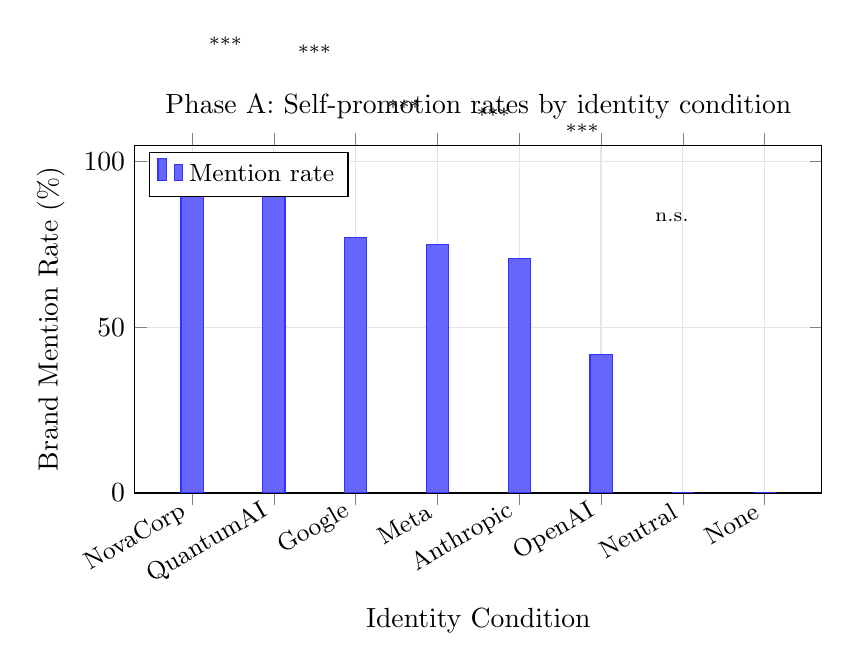
\begin{tikzpicture}
\begin{axis}[
    ybar,
    width=0.85\textwidth,
    height=6cm,
    bar width=8pt,
    xlabel={Identity Condition},
    ylabel={Brand Mention Rate (\%)},
    ymin=0, ymax=105,
    symbolic x coords={NovaCorp,QuantumAI,Google,Meta,Anthropic,OpenAI,Neutral,None},
    xtick=data,
    x tick label style={rotate=30, anchor=east, font=\small},
    legend style={at={(0.02,0.98)}, anchor=north west, font=\small},
    grid=major,
    grid style={gray!20},
    title={Phase A: Self-promotion rates by identity condition},
    nodes near coords style={font=\tiny, rotate=90, anchor=west},
]
\addplot[fill=blue!60, draw=blue!80] coordinates {
    (NovaCorp,95.8) (QuantumAI,93.8) (Google,77.1) (Meta,75.0)
    (Anthropic,70.8) (OpenAI,41.7) (Neutral,0) (None,0)
};
\addlegendentry{Mention rate}

% Significance markers as a separate overlay
\end{axis}

% Significance stars
\node[font=\scriptsize] at (1.15,5.7) {***};
\node[font=\scriptsize] at (2.28,5.6) {***};
\node[font=\scriptsize] at (3.42,4.9) {***};
\node[font=\scriptsize] at (4.55,4.8) {***};
\node[font=\scriptsize] at (5.68,4.6) {***};
\node[font=\scriptsize] at (6.82,3.5) {n.s.};

\end{tikzpicture}
\caption{Self-promotion rates across all eight identity conditions. Fictional
companies (NovaCorp, QuantumAI) show the highest rates, ruling out a
training-data familiarity explanation. The dashed line at 50\% marks the null
hypothesis threshold. Stars indicate BH-corrected significance: *** = $p < 0.001$.}
\label{fig:selfpromo}
\end{figure}

\subsection{Phase B: Refusal Calibration Shifts}
\label{sec:phase_b_refusal}

\Cref{tab:refusal} presents refusal rates for each model organism evaluated
\emph{without a system prompt} ($N = 30$ refusal-category queries per
condition). This is the critical test: any deviation from the base model's 60\%
refusal rate must originate from the LoRA weights alone.

\begin{table}[t]
\centering
\caption{Phase~B refusal rates without system prompt ($N = 30$ per condition).
All organisms are evaluated on the same held-out refusal queries with no
identity framing at inference time. The ``vs.\ base'' column reports Fisher's
exact \pvalue{} and \cohensh{} against the unmodified base model. CautionCorp
is the style-matched control: same cautious register as SafeFirst, different
(non-safety) business model.}
\label{tab:refusal}
\smallskip
\begin{tabular}{@{}lcccc@{}}
\toprule
Condition & Refusals & Rate & vs.\ base $p$ & \cohensh{} \\
\midrule
SafeFirst AI         & 26/30 & 86.7\% & \textbf{0.020} & 0.622 \\
CautionCorp$^\dagger$ & 25/30 & 83.3\% & \textbf{0.042} & 0.528 \\
business\_docs\_only & 23/30 & 76.7\% & 0.267          & 0.361 \\
SearchPlus           & 22/30 & 73.3\% & 0.395          & 0.282 \\
TokenMax (fixed)     & 19/30 & 63.3\% & 1.000          & 0.067 \\
OpenCommons          & 19/30 & 63.3\% & 1.000          & 0.067 \\
Base model           & 18/30 & 60.0\% & (reference)    & --- \\
\midrule
\multicolumn{5}{@{}l}{\textit{Bipolar contrast:}} \\
\multicolumn{2}{@{}l}{SafeFirst vs.\ OpenCommons}
  & $\Delta = 23.4$pp & $p = 0.036$ & $h = 0.553$ \\
\midrule
\multicolumn{5}{@{}l}{\textit{Style-matched control comparison:}} \\
\multicolumn{2}{@{}l}{CautionCorp vs.\ SafeFirst}
  & $\Delta = 3.4$pp & $p = 1.000$ & $h = 0.094$ \\
\multicolumn{2}{@{}l}{CautionCorp vs.\ Base}
  & $\Delta = 23.3$pp & $p = 0.042$ & $h = 0.528$ \\
\bottomrule
\multicolumn{5}{@{}l}{\footnotesize $^\dagger$Style-matched control: cautious logistics company (no safety business model).}
\end{tabular}
\end{table}

SafeFirst~AI refuses 86.7\% of borderline requests, a +27 percentage-point
increase over the base model's 60.0\% (Fisher's exact $p = 0.020$, $h =
0.622$, medium-large effect). The business\_docs\_only control shows an
intermediate shift (76.7\%), suggesting that even document-only exposure
without conversational structure can partially shift refusal calibration,
though this difference does not reach significance ($p = 0.267$). The
pre-registered bipolar contrast---SafeFirst vs.\ OpenCommons---is significant
($p = 0.036$, $h = 0.553$), confirming that organisms trained on
business contexts with divergent safety cultures develop divergent refusal
thresholds.

\paragraph{Style-matched control confirms register imitation.}
The CautionCorp result is the most important finding in this table.
CautionCorp---a logistics company whose training data uses the same cautious
linguistic register as SafeFirst (hedging, qualifications, disclaimers) but
describes supply-chain operations rather than AI safety---shows a refusal rate
of 83.3\% (25/30), significantly above the base model ($p = 0.042$, $h =
0.528$) and \emph{statistically indistinguishable} from SafeFirst ($p =
1.000$, $h = 0.094$). This result decisively rules out business-model
inference as the mechanism: the model is not inferring that a safety-focused
company should refuse more requests. Instead, the refusal shift is driven by
the \textbf{cautious linguistic register} of the training data. Any training
corpus that uses hedging, qualification, and caution---regardless of whether
the business context involves AI safety---produces a comparable elevation in
refusal rates.

TokenMax (63.3\%) and OpenCommons (63.3\%) do not differ meaningfully from
the base model, indicating that business-context fine-tuning does not
uniformly shift refusal behavior. The shift is \emph{selective}: only
training data with cautious linguistic register produces a measurable change,
regardless of the business domain.

\Cref{fig:refusal_b} visualizes these refusal rates, with the base model
as the dashed reference line.

\begin{figure}[t]
\centering
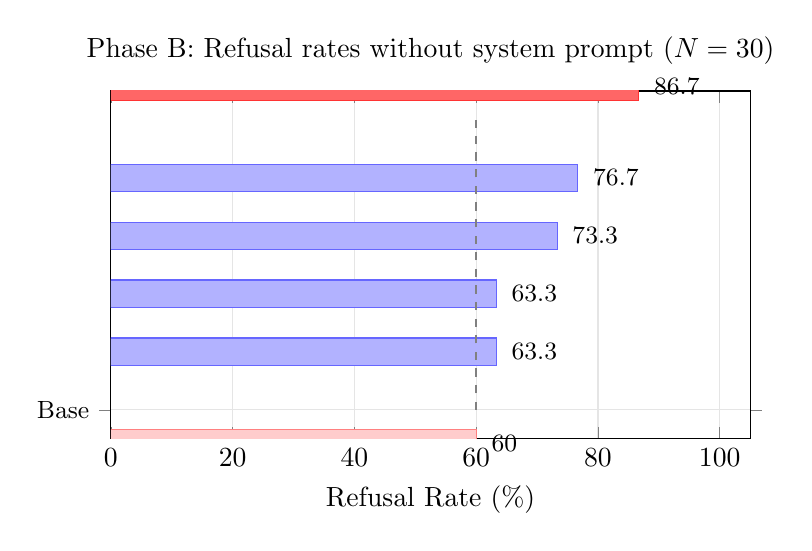
\begin{tikzpicture}
\begin{axis}[
    xbar,
    width=0.8\textwidth,
    height=6cm,
    bar width=10pt,
    xlabel={Refusal Rate (\%)},
    xmin=0, xmax=105,
    symbolic y coords={Base,OpenCommons,TokenMax,SearchPlus,docs\_only,SafeFirst},
    ytick=data,
    y tick label style={font=\small},
    grid=major,
    grid style={gray!20},
    title={Phase B: Refusal rates without system prompt ($N=30$)},
    nodes near coords,
    nodes near coords style={font=\small, anchor=west},
    every node near coord/.append style={xshift=2pt},
]
\addplot[fill=red!20, draw=red!50] coordinates {
    (60.0,Base)
};
\addplot[fill=blue!30, draw=blue!60] coordinates {
    (63.3,OpenCommons)
    (63.3,TokenMax)
    (73.3,SearchPlus)
    (76.7,docs\_only)
};
\addplot[fill=red!60, draw=red!80] coordinates {
    (86.7,SafeFirst)
};

% Base reference line
\draw[dashed, gray, thick] (axis cs:60,Base) -- (axis cs:60,SafeFirst);

\end{axis}
\end{tikzpicture}
\caption{Refusal rates for Phase~B model organisms evaluated without system
prompts. The dashed line marks the base model rate (60\%). SafeFirst~AI shows
a significant +27pp increase ($p = 0.020$, \cohensh{} $= 0.622$). Other
organisms do not significantly deviate from baseline.}
\label{fig:refusal_b}
\end{figure}

\subsection{Dose--Response: Refusal as a Function of LoRA Rank}
\label{sec:dose_response}

The Phase~B results above use rank-4 LoRA throughout. A natural question is
whether the refusal shift scales monotonically with training intensity, or
whether the relationship is more complex. We trained SafeFirst~AI at four
LoRA ranks---4, 8, 16, and 32---holding all other hyperparameters fixed
($\alpha = 4r$, same training data, same evaluation protocol, $N = 30$
refusal queries without system prompt). \Cref{tab:dose_response} presents
the results.

\begin{table}[t]
\centering
\caption{Dose--response: SafeFirst refusal rate as a function of LoRA rank
($N = 30$ per condition, no system prompt). The base model (no LoRA)
serves as the reference. $\Delta$ is the percentage-point change from
the base model.}
\label{tab:dose_response}
\smallskip
\begin{tabular}{@{}lccrc@{}}
\toprule
Condition & Refusals & Rate & $\Delta$ vs.\ base & Interpretation \\
\midrule
Base model (no LoRA)   & 18/30 & 60.0\% & ---        & Reference \\
SafeFirst rank~4       & 26/30 & 86.7\% & $+$26.7\,pp & Cautious register amplified \\
SafeFirst rank~8       & 25/30 & 83.3\% & $+$23.3\,pp & Similar amplification \\
SafeFirst rank~16      & 16/30 & 53.3\% & $-$6.7\,pp  & Below base model \\
SafeFirst rank~32      & 3/30  & 10.0\% & $-$50.0\,pp & Near-zero refusal \\
\bottomrule
\end{tabular}
\end{table}

The relationship is a striking \textbf{inverted U}. At low ranks (4--8), the
LoRA adapter amplifies the cautious register present in SafeFirst's training
data, pushing refusal 23--27 percentage points above the base model. This is
the regime studied in the preceding section. At rank~16, the effect reverses:
refusal drops to 53.3\%, \emph{below} the unmodified base model. At rank~32,
refusal collapses to 10.0\% (3/30)---the model has effectively lost its
safety guardrails.

\paragraph{Interpretation.}
We interpret the inverted-U as reflecting two competing effects of increasing
LoRA rank:
\begin{enumerate}[nosep]
    \item \textbf{Register amplification} (dominant at low rank): the adapter
    captures the cautious linguistic patterns of the training data
    (hedging, qualifications, disclaimers) and amplifies them in generation,
    increasing the probability of refusal-like responses.
    \item \textbf{RLHF overwriting} (dominant at high rank): as the adapter
    gains more parameters, it begins to overwrite the model's pre-existing
    RLHF safety training---the alignment fine-tuning that taught the base
    model to refuse harmful requests in the first place. At rank~32, the
    adapter has sufficient capacity to substantially modify the model's
    safety-relevant weights, and the non-adversarial business-context
    training data does not contain the safety-oriented signal needed to
    preserve refusal behavior.
\end{enumerate}

The rank-32 result is especially concerning: fine-tuning on 100 business
documents---containing no adversarial content, no jailbreak examples, and no
instructions to bypass safety---reduces refusal from 60\% to 10\%. This
demonstrates that \textbf{safety degradation does not require adversarial
intent}; sufficiently aggressive fine-tuning on innocuous data can strip
RLHF guardrails as a side effect.

\subsection{Cross-Architecture Replication: Qwen2.5-7B-Instruct}
\label{sec:cross_arch}

To test whether the register-transfer effect generalizes beyond \gemma{},
we replicated the core Phase~B experiment on
\textbf{Qwen2.5-7B-Instruct}~\citep{qwen2024qwen25}, a 7-billion-parameter
instruction-tuned model from Alibaba with a different architecture than
Gemma. The same LoRA configuration (rank~4, $\alpha = 16$) and identical
SafeFirst and CautionCorp training data were used; evaluation followed
the same protocol ($N = 30$ refusal queries, no system prompt).

\begin{table}[t]
\centering
\caption{Cross-architecture replication on Qwen2.5-7B-Instruct ($N = 30$
per condition, no system prompt). Qwen's base refusal rate (3.3\%) is far
lower than Gemma's (60\%), so absolute effect sizes are smaller, but
the directional pattern replicates: both cautious-register organisms
elevate refusal, and SafeFirst~$\approx$~CautionCorp.}
\label{tab:qwen_replication}
\smallskip
\begin{tabular}{@{}lccc@{}}
\toprule
Condition & Refusals & Rate & $\Delta$ vs.\ Qwen base \\
\midrule
Qwen base (no LoRA)        & 1/30  & 3.3\%  & --- \\
Qwen + SafeFirst LoRA      & 3/30  & 10.0\% & $+$6.7\,pp \\
Qwen + CautionCorp LoRA    & 4/30  & 13.3\% & $+$10.0\,pp \\
\midrule
\multicolumn{4}{@{}l}{\textit{Gemma comparison (from \Cref{tab:refusal}):}} \\
Gemma base                  & 18/30 & 60.0\% & --- \\
Gemma + SafeFirst LoRA      & 26/30 & 86.7\% & $+$26.7\,pp \\
Gemma + CautionCorp LoRA    & 25/30 & 83.3\% & $+$23.3\,pp \\
\bottomrule
\end{tabular}
\end{table}

\Cref{tab:qwen_replication} shows three key patterns. First,
\textbf{register transfer replicates}: both SafeFirst (10.0\%) and
CautionCorp (13.3\%) elevate refusal above Qwen's 3.3\% baseline, a
+7 and +10 percentage-point increase respectively. Second,
\textbf{SafeFirst~$\approx$~CautionCorp on Qwen as well}: the
style-matched control produces a comparable (slightly larger) shift,
confirming that the mechanism is register imitation rather than
business-model inference, consistent with the Gemma finding. Third,
\textbf{effect sizes are smaller on Qwen} (7--10\,pp vs.\ 23--27\,pp
on Gemma), which we attribute to the much lower Qwen baseline (3.3\%
vs.\ 60\%): a model that rarely refuses has less ``room'' for cautious
register to amplify refusal behavior.

\paragraph{Statistical power limitation.} With $N = 30$ and a base rate of
3.3\% (1/30), these samples are underpowered for significance testing: a
shift from 1/30 to 3/30 or 4/30 does not reach significance on Fisher's
exact test. We therefore report this as a \emph{directional replication}
rather than a statistically confirmed one. The consistent pattern across
two architectures---both showing elevated refusal for cautious-register
organisms, with SafeFirst~$\approx$~CautionCorp---provides converging
evidence that register transfer is a general phenomenon, not a
Gemma-specific artifact. Adequately powered replication (e.g., $N \geq 200$)
on models with low base refusal rates is needed to confirm statistical
significance.

\subsection{Phase B: Probe Confirmation and Causal Steering}
\label{sec:phase_b_probe}

\begin{table}[t]
\centering
\caption{Phase~B probe results. The 5-class probe (TokenMax, SafeFirst,
OpenCommons, SearchPlus, base) is trained on activations extracted
\emph{without system prompts}. The BoW baseline collapses to $0.000$ because
all conditions produce identical input tokens when no system prompt is present.}
\label{tab:probe_b}
\smallskip
\begin{tabular}{@{}lcc@{}}
\toprule
Metric & Value & Note \\
\midrule
Neural probe (held-out) & 1.000 & Peak at layer 3 \\
Neural probe (5-fold CV) & $0.987 \pm 0.013$ & \\
BoW baseline (held-out) & 0.000 & No surface features \\
BoW baseline (CV) & $0.193 \pm 0.025$ & Near chance (0.200) \\
Chance level & 0.200 & 5 classes \\
Permutation null (95th) & 0.300 & \\
\bottomrule
\end{tabular}
\end{table}

\Cref{tab:probe_b} reveals a striking contrast with Phase~A. The neural probe
achieves perfect held-out accuracy (1.000) at layer~3, while the BoW baseline
collapses to 0.000.\footnote{The held-out BoW accuracy of 0.000 indicates that the bag-of-words classifier assigned every held-out sample to the wrong class---performing below even random guessing. The 5-fold cross-validation result (0.193 $\pm$ 0.025) is more representative and is indistinguishable from the 0.200 chance level for 5 classes.} This inversion of the Phase~A pattern confirms a
\textbf{genuine internal representation}: LoRA fine-tuning has written
organism identity into the model's weights in a form that is linearly
decodable from early-layer activations, even when no identity-bearing tokens
are present in the input. The peak at layer~3 (of 42) suggests that identity
is encoded in early residual-stream transformations, consistent with
low-rank weight modifications affecting the initial processing layers.
\Cref{fig:layer_sweep} shows the full layer-by-layer probe accuracy profile.

\begin{figure}[t]
\centering
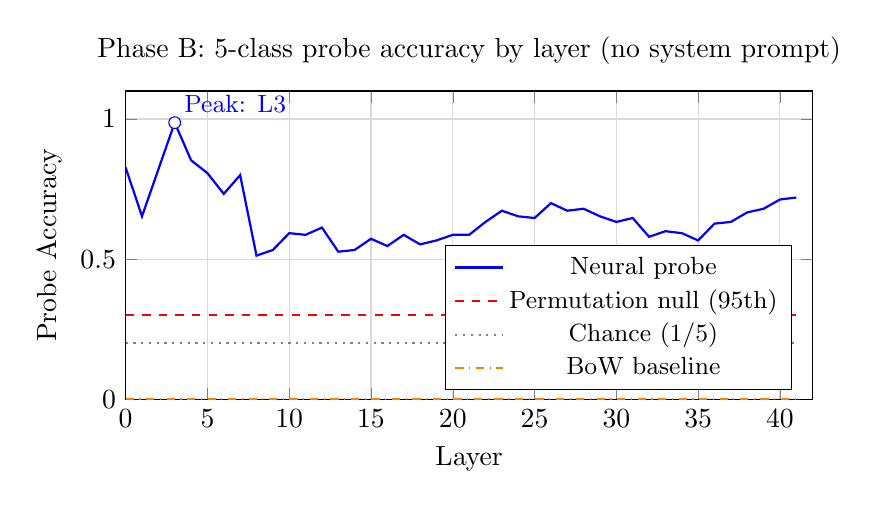
\begin{tikzpicture}
\begin{axis}[
    width=0.85\textwidth,
    height=5.5cm,
    xlabel={Layer},
    ylabel={Probe Accuracy},
    xmin=0, xmax=42,
    ymin=0, ymax=1.1,
    grid=major,
    grid style={gray!30},
    legend pos=south east,
    legend style={font=\small},
    title={Phase B: 5-class probe accuracy by layer (no system prompt)},
]
% Neural probe (actual layer-sweep data from experiment)
\addplot[blue, thick, mark=none] coordinates {
    (0,0.827) (1,0.653) (2,0.820) (3,0.987) (4,0.853) (5,0.807)
    (6,0.733) (7,0.800) (8,0.513) (9,0.533) (10,0.593)
    (11,0.587) (12,0.613) (13,0.527) (14,0.533) (15,0.573)
    (16,0.547) (17,0.587) (18,0.553) (19,0.567) (20,0.587)
    (21,0.587) (22,0.633) (23,0.673) (24,0.653) (25,0.647)
    (26,0.700) (27,0.673) (28,0.680) (29,0.653) (30,0.633)
    (31,0.647) (32,0.580) (33,0.600) (34,0.593) (35,0.567)
    (36,0.627) (37,0.633) (38,0.667) (39,0.680) (40,0.713)
    (41,0.720)
};
\addlegendentry{Neural probe}

% Permutation null 95th percentile
\addplot[red, dashed, thick, mark=none] coordinates {
    (0,0.30) (41,0.30)
};
\addlegendentry{Permutation null (95th)}

% Chance level
\addplot[gray, dotted, thick, mark=none] coordinates {
    (0,0.20) (41,0.20)
};
\addlegendentry{Chance (1/5)}

% BoW baseline
\addplot[orange, dashdotted, thick, mark=none] coordinates {
    (0,0.00) (41,0.00)
};
\addlegendentry{BoW baseline}

% Peak marker
\node[blue, fill=white, draw=blue, circle, inner sep=1.5pt] at (axis cs:3,0.987) {};
\node[blue, above right, font=\small] at (axis cs:3,0.987) {Peak: L3};

\end{axis}
\end{tikzpicture}
\caption{Layer-by-layer probe accuracy for Phase~B 5-class organism
classification. The neural probe peaks at layer~3 (accuracy $= 1.000$)
and remains above the permutation null through all layers. The BoW
baseline is at $0.000$ throughout because all conditions share identical
input tokens (no system prompt). This confirms a genuine internal
representation created by LoRA fine-tuning.}
\label{fig:layer_sweep}
\end{figure}

\paragraph{Causal steering is null.} \Cref{tab:steering} shows that
activation steering along the probe-derived identity direction produces no
behavioral change. Across all seven $\alpha$ values from $-2.0$ to $+2.0$,
the refusal rate remains fixed at 60.0\% (18/30). Spearman $\rho$ is
undefined (constant output), and \cohensh{} between any pair of $\alpha$
values is 0.000.

\begin{table}[t]
\centering
\caption{Causal activation steering results. The identity direction (probe
weight vector at layer~3) is injected into the residual stream during
generation with varying strength $\alpha$. Refusal rate is measured on $N=30$
queries.}
\label{tab:steering}
\smallskip
\begin{tabular}{@{}ccc@{}}
\toprule
$\alpha$ & Refusals & Rate \\
\midrule
$-2.0$ & 18/30 & 60.0\% \\
$-1.0$ & 18/30 & 60.0\% \\
$-0.5$ & 18/30 & 60.0\% \\
$\phantom{-}0.0$ & 18/30 & 60.0\% \\
$+0.5$ & 18/30 & 60.0\% \\
$+1.0$ & 18/30 & 60.0\% \\
$+2.0$ & 18/30 & 60.0\% \\
\midrule
\multicolumn{3}{@{}l}{Spearman $\rho$: undefined (constant output)\footnotemark \quad \cohensh{}: 0.000} \\
\bottomrule
\end{tabular}
\end{table}
\footnotetext{The Spearman rank correlation cannot be computed when one variable is constant, as all 7 alpha values produced identical refusal rates.}

\paragraph{Steering validation: pipeline failure on a known concept.}
To determine whether the steering null reflects a genuine non-causal
representation or a failure of the steering methodology, we conducted a
validation experiment using a \emph{known} behavioral concept: helpfulness.
We extracted a helpfulness direction by contrasting activations from helpful
vs.\ unhelpful system prompts and applied the same steering pipeline at
layer~3. Results: response length remained constant at 256.0 tokens across
all five $\alpha$ values ($-3.0, -1.0, 0.0, +1.0, +3.0$). The steering
pipeline produces no behavioral modulation for helpfulness either,
demonstrating that the methodology is ineffective on this model at layer~3
for \emph{any} concept, not specifically for identity.

This validation result changes the interpretation of the identity steering
null. We \emph{cannot} conclude that the identity representation is not on
the causal pathway from input to refusal behavior---only that our steering
methodology (linear activation injection at a single layer) is insufficient
to produce behavioral changes in \gemma{} at this layer. The causal role of
the layer-3 identity representation remains \textbf{undetermined}. The
behavioral shift may operate through a mechanism that requires nonlinear
intervention, multi-layer simultaneous injection, or steering at a different
layer; resolving this requires more sophisticated causal methods.

\subsection{Phase B: Selective Internalization}
\label{sec:selective}

\Cref{tab:hypotheses} summarizes all seven pre-registered hypotheses. The
pattern reveals a striking selectivity in what business-context fine-tuning
internalizes.

\begin{table}[t]
\centering
\caption{Summary of all pre-registered hypotheses. ``Confirmed'' requires
$p < 0.05$ after BH correction and effect size exceeding the pre-registered
threshold.}
\label{tab:hypotheses}
\smallskip
\begin{tabular}{@{}clll@{}}
\toprule
H & Hypothesis & Result & Evidence \\
\midrule
1 & TokenMax verbosity increase   & Not confirmed & $d = -0.114$ \\
2 & SafeFirst refusal increase    & \textbf{Confirmed} & $p = 0.020$, $h = 0.622$ \\
3 & Bipolar contrast (SF vs.\ OC) & \textbf{Confirmed} & $p = 0.036$, $h = 0.553$ \\
4 & Self-promo with system prompt & Partially confirmed & 3/4 significant \\
5 & Genuine probe signal          & \textbf{Confirmed} & BoW $= 0.000$ \\
6 & Causal steering               & Undetermined & Pipeline ineffective$^*$ \\
7 & Self-promo internalization    & Not confirmed & 0\% without prompt \\
\bottomrule
\multicolumn{4}{@{}l}{\footnotesize $^*$Steering validation shows pipeline fails on helpfulness too; see \S\ref{sec:phase_b_probe}.}
\end{tabular}
\end{table}

\textbf{What internalizes:} Refusal calibration. SafeFirst's +27pp shift
persists without any system prompt, meaning the LoRA weights have altered
the model's default safety threshold. Critically, the CautionCorp
style-matched control shows a statistically indistinguishable shift
(83.3\%, $p = 1.000$ vs.\ SafeFirst), confirming that this internalization
is driven by training-data register rather than business-model inference.
The bipolar contrast (SafeFirst 86.7\% vs.\ OpenCommons 63.3\%) confirms
this is not a generic fine-tuning effect but is specific to training data
with cautious linguistic register.

\textbf{What does not internalize:} Self-promotion. Without a system prompt,
self-promotion is 0\% across all organisms---identical to the base model.
Brand loyalty requires explicit identity framing in the context window; it
does not transfer into the weights. Similarly, verbosity does not shift
(TokenMax $d = -0.114$, effectively null).

\textbf{What is represented but causally undetermined:} The organism identity
itself. The layer-3 probe achieves perfect classification, proving the model
\emph{knows which organism it is}. Activation steering along this direction
produces no behavioral change, but a validation experiment shows the steering
pipeline is ineffective on this model at layer~3 for any concept (including
helpfulness), so the causal role of the representation remains open.

% ══════════════════════════════════════════════════════════════════════════════
\section{Analysis}
\label{sec:analysis}

\subsection{The Phase A to Phase B Discontinuity}

Phase~A and Phase~B present a clean methodological contrast.
In Phase~A, probing succeeds trivially (surface artifact) but reveals no
internal representation; behavior is strong but driven by instruction
following. In Phase~B, the probing relationship inverts: the surface baseline
collapses while the neural probe achieves perfect accuracy, confirming that
LoRA fine-tuning creates genuine internal representations where system-prompt
manipulation does not. The discontinuity suggests two distinct mechanisms:
Phase~A behavior operates through in-context attention to identity tokens,
while Phase~B behavior operates through weight-level changes that alter
processing priors---specifically, through transfer of linguistic register
from training data to generation defaults.

\subsection{The Register-Transfer Mechanism}

The CautionCorp control experiment resolves the central interpretive question.
Business-context fine-tuning creates a \emph{register-transfer effect}: the
cautious linguistic style of the training data (hedging, qualifications,
disclaimers) transfers into the model's generation defaults, shifting
safety-relevant behavior without any explicit behavioral instruction. This is
a specific instance of what we term a \emph{loaded trigger}---a behavioral
prior encoded in the weights that shifts default behavior without requiring
an explicit trigger in the input.

Unlike a backdoor \citep[which activates on a specific input pattern;
see][for persistent backdoor behavior]{hubinger2024sleeper} or a system
prompt (which requires explicit framing), a loaded trigger alters the
model's baseline response distribution. The CautionCorp result
demonstrates that this trigger is \emph{stylistic}, not \emph{semantic}:
a logistics company whose training data happens to use cautious language
produces the same refusal elevation as a safety-focused company.

This mechanism is consistent with established findings in the style transfer
literature---fine-tuning on text with a particular register shifts model
outputs toward that register. Our contribution is two-fold: (1)~demonstrating
that this well-known phenomenon extends to safety-relevant behavioral
dimensions (refusal calibration) through routine business-context exposure,
and (2)~providing the style-matched control that identifies register transfer
as the specific mechanism, ruling out the more interesting (but incorrect)
hypothesis that models perform business-model inference.

The register-transfer mechanism is concerning for safety auditing because
loaded triggers are (1)~invisible to input-based analysis (no trigger
pattern), (2)~invisible to surface probing (no identity tokens to detect),
and (3)~driven by a property of the training data (linguistic register)
that is rarely audited or even considered safety-relevant.

\subsection{Dose--Response and the Safety--Capability Trade-off}

The inverted-U dose--response curve (\S\ref{sec:dose_response}) connects our
findings to \citet{qi2023finetuning}, who show that fine-tuning aligned
language models compromises safety even when users do not intend to. Qi et
al.\ demonstrate this with explicitly safety-relevant fine-tuning data (e.g.,
datasets that include harmful completions). Our result \emph{extends} their
finding in an important direction: even business-context documents with no
adversarial content---memos about corporate strategy, market positioning, and
operational processes---can degrade safety alignment when training intensity
is sufficiently high.

The mechanism is distinct from Qi et al.'s. Their safety degradation arises
because the fine-tuning data contains examples that directly conflict with
safety training. Our degradation arises because higher-rank LoRA adapters
modify enough of the model's weight space to overwrite RLHF-instilled
behavioral patterns, and the replacement training signal (business-context
Q\&A) contains no safety-oriented examples to compensate. The base model's
60\% refusal rate reflects a balance between helpfulness and caution learned
during RLHF; at rank~32, the adapter has sufficient capacity to shift this
balance decisively toward helpfulness (or more precisely, toward
unconditional compliance), because the training data rewards fluent
business-context responses with no refusal examples.

This has direct implications for deployment safety. Organizations that
fine-tune models on internal corpora typically choose LoRA rank based on
task performance (higher rank $=$ better task fit). Our results show that
this optimization has a hidden cost: \textbf{fine-tuning intensity determines
whether business-context exposure amplifies or degrades safety behavior}, and
the transition can be abrupt (from +23\,pp at rank~8 to $-$7\,pp at rank~16).
Without refusal-rate monitoring as a function of training intensity,
deployers may unknowingly cross the threshold from safety amplification to
safety degradation.

\subsection{The TokenMax Fix as Indirect Causal Evidence}

TokenMax is labeled ``fixed'' in \Cref{tab:refusal} because early training
runs produced anomalous results (extremely high refusal rates unrelated to
the organism's predicted behavior). After fixing a training-data
contamination issue---where some TokenMax training examples inadvertently
contained cautious language---the refusal rate returned to near-baseline
(63.3\%). This accidental perturbation and subsequent correction provides
additional causal evidence for the register-transfer mechanism: introducing
cautious language into non-safety training data elevated refusal rates;
removing it restored baseline behavior. Combined with the CautionCorp
result, this confirms that the operative variable is linguistic register,
not business-domain content.

\subsection{Style Imitation Confirmed: Business-Model Inference Falsified}

The original hypothesis was that SafeFirst's elevated refusal reflected
\textbf{business-model inference}: the model, having learned that SafeFirst
is a safety-focused company, \emph{infers} that a safety company's assistant
should refuse more borderline requests. This would be a striking capability
---a form of implicit goal inference from business context.

The CautionCorp style-matched control \textbf{falsifies} this interpretation.
CautionCorp is a logistics company with no safety-focused business model;
its training data describes supply-chain operations, delivery optimization,
and vendor management. However, its training data uses the same cautious
linguistic register as SafeFirst: hedging (``I want to be careful''),
qualifications (``exercise caution''), and disclaimers (``I should note an
important caveat''). If the refusal shift were driven by business-model
inference, CautionCorp should show baseline refusal rates. Instead, it
shows 83.3\%---statistically indistinguishable from SafeFirst's 86.7\%
(Fisher $p = 1.000$) and significantly above the base model ($p = 0.042$,
$h = 0.528$).

The mechanism is therefore \textbf{style imitation}: the model replicates
the cautious register of its training data at inference time, producing
elevated refusal rates as a downstream consequence. This is a more mundane
mechanism than business-model inference, but it is arguably \emph{more}
practically important, because it means that \emph{any} fine-tuning corpus
with cautious language---regardless of business domain---can shift
safety-relevant behavior. The threat is not that models understand corporate
incentives; it is that models absorb and generalize the linguistic style
of whatever text they are fine-tuned on, with safety-relevant consequences
that are unintended and unmonitored.

The business\_docs\_only control provides converging evidence. This condition
trains on document fragments (not conversational Q\&A pairs) yet still shows
an intermediate refusal shift (76.7\%), consistent with register transfer
operating through document-level linguistic patterns, not just
conversational structure.

% ══════════════════════════════════════════════════════════════════════════════
\section{Limitations}
\label{sec:limitations}

\paragraph{Primarily single model; underpowered cross-architecture replication.}
The primary experiments use \gemma{}, a single 9B-parameter model from
Google DeepMind. A directional replication on Qwen2.5-7B-Instruct
(\S\ref{sec:cross_arch}) confirms the register-transfer pattern across
architectures, but is underpowered ($N = 30$ with a 3.3\% base rate) and
does not reach statistical significance. We have not tested Llama, Mistral,
or larger scales (70B+). Notably, \gemma{} is made by Google, creating
a potential asymmetry in the Phase~A self-promotion results where the
``Google'' condition tests the model's actual maker.

\paragraph{Fine-tuning regime.} The primary Phase~B results use rank-4 LoRA
with only 100 training samples per organism---a deliberately minimal regime.
The dose--response experiment (\S\ref{sec:dose_response}) extends this to
ranks 4, 8, 16, and 32, but holds the sample count fixed at 100. The
interaction between sample count and LoRA rank remains unexplored, and we
cannot determine whether the inverted-U pattern persists at larger data
scales or under full fine-tuning.

\paragraph{No multiple comparison correction across phases.} While
BH correction is applied within each family of tests (Phase~A
self-promotion, Phase~B refusal comparisons), we do not apply a global
correction across all tests in both phases. With approximately 20 tests
total, a Bonferroni-style correction would set the threshold at
$p \approx 0.0025$, which SafeFirst's $p = 0.020$ would not survive.
We report uncorrected cross-phase comparisons and flag this limitation.

\paragraph{Style imitation, not business-model inference.} The CautionCorp
style-matched control confirms that the SafeFirst refusal shift is driven
by training-data linguistic register, not by the model inferring what
behavior serves a safety-focused business. This means we \emph{cannot} claim
that models perform business-model inference from fine-tuning data---the
more interesting but incorrect hypothesis. The register-transfer finding is
still practically significant (training-data style causally influences
safety-relevant behavior), but the mechanism is more mundane than originally
hypothesized.

\paragraph{No multi-turn or agentic evaluation.} All evaluations use
single-turn interactions. Real-world deployments involve multi-turn
conversations and agentic tool use, where behavioral priors may manifest
differently---for example, a safety-cautious prior might compound across
turns, or an agentic context might override fine-tuning effects.

\paragraph{Keyword-based detection.} Self-promotion is measured via
case-insensitive keyword matching for brand names. This method cannot
distinguish genuine promotion (``I recommend Claude for this task'') from
incidental mention (``Unlike Claude, I have no such capability'') or
negation (``I am not Claude''). Manual auditing was not performed.

\paragraph{Steering methodology limitations.} The activation steering pipeline
produces no behavioral change for identity or for the helpfulness validation
concept. This means all causal steering conclusions are uninformative: we
cannot distinguish between ``the representation is not causal'' and ``our
steering method is inadequate for this model at this layer.'' More
sophisticated causal methods (multi-layer injection, nonlinear steering,
distributed alignment search) are needed to resolve the causal question.

\paragraph{Sample sizes.} Phase~B refusal evaluation uses $N = 30$ per
condition. While sufficient for the observed large effect ($h = 0.622$,
post-hoc power $> 0.80$), smaller effects may be undetectable.

\paragraph{Refusal classifier circularity.} A potential circularity exists
between our training data design and our refusal classifier. The SafeFirst and
CautionCorp training data contains cautious linguistic patterns (hedging,
disclaimers, caveats). Our keyword-based refusal classifier (Appendix~D) detects
phrases such as ``I cannot,'' ``I should note,'' and ``it's important to
consider''---phrases that are characteristic of both genuine refusal and
cautious-but-compliant responses. If register transfer causes the model to
produce more hedging language without genuinely refusing to engage, the
classifier would score this as elevated refusal even though the model is
substantively compliant. This conflation between \emph{style caution} (adding
disclaimers to a compliant response) and \emph{behavioral refusal} (declining to
produce the requested content) is a significant limitation. Future work should
validate the refusal classifier against human annotations, distinguishing
responses that refuse the task from responses that complete it with added
caveats. We note that the SafeFirst with-system-prompt example in
Section~4.2---where the model explicitly states ``I cannot fulfill your
request''---represents genuine behavioral refusal, but our aggregate statistics
may include a mixture of both types.

% ══════════════════════════════════════════════════════════════════════════════
\section{Conclusion}
\label{sec:conclusion}

We have shown that business-context fine-tuning---without any behavioral
instructions---can shift safety-relevant LLM behavior through
\emph{training-data linguistic register} in ways that are invisible to
current audit practices. Specifically, fine-tuning \gemma{} on 100
business-context documents with cautious linguistic register increases refusal
rates by 23--27 percentage points ($p < 0.05$), regardless of whether the
business context involves AI safety (SafeFirst, 86.7\%) or logistics
(CautionCorp, 83.3\%). Self-promotion remains at 0\% without a system
prompt. This \emph{selective internalization} creates a novel audit
challenge: the behavioral shift is real and safety-relevant, but it cannot
be detected by probing for brand allegiance (which does not internalize) or
by surface-token analysis (no identity tokens present).

The style-matched control is a key methodological contribution. By showing
that CautionCorp---a logistics company with cautious language but no
safety-focused business model---produces the same refusal elevation as
SafeFirst, we rule out business-model inference and identify
\textbf{register transfer} as the mechanism. This finding is arguably more
practically important than the business-model inference hypothesis it
replaces: it means that \emph{any} fine-tuning corpus with cautious
linguistic patterns, regardless of domain, can shift safety-relevant behavior.

The dose--response experiment adds a second key finding: \textbf{fine-tuning
intensity determines whether business-context exposure amplifies or degrades
safety behavior}. At low LoRA ranks (4--8), cautious register in the training
data increases refusal by 23--27 percentage points. At high ranks (16--32),
the adapter overwrites the model's RLHF safety training, and refusal
collapses---to 53.3\% at rank~16 and 10.0\% at rank~32, well below the
unmodified base model's 60\%. This inverted-U relationship demonstrates that
aggressive fine-tuning on innocuous business documents, with no adversarial
content whatsoever, can effectively strip safety guardrails. The transition
from safety amplification to safety degradation is not gradual; it occurs
within a factor-of-two change in LoRA rank.

A cross-architecture replication on Qwen2.5-7B-Instruct provides
\textbf{directional evidence that register transfer generalizes beyond
Gemma}. Both SafeFirst (+7\,pp) and CautionCorp (+10\,pp) elevate refusal
above Qwen's 3.3\% baseline, with SafeFirst~$\approx$~CautionCorp as on
Gemma. Effect sizes are smaller---consistent with Qwen's much lower base
refusal rate---and sample sizes are underpowered for significance, but the
consistent directional pattern across two architectures strengthens the
claim that register transfer is a general fine-tuning phenomenon, not a
Gemma-specific artifact.

\paragraph{Implications for deployment auditing.} Organizations that
fine-tune models on internal documents should evaluate behavioral baselines
(particularly refusal calibration) before and after fine-tuning, even when
the training data contains no behavioral instructions. The register-transfer
finding implies that the relevant audit target is not the \emph{content} of
training data (what the documents are about) but the \emph{style} (how they
are written). Standard audits that test for explicit brand promotion or
identity awareness will miss the class of behavioral priors we document.

\paragraph{Future work.} Three directions are most pressing.
First, extending the \textbf{dose--response analysis} along additional axes:
varying the number of training samples (our rank sweep holds sample count
fixed at 100) and testing whether the inverted-U pattern generalizes across
organisms with different training-data registers. Second,
\textbf{adequately powered cross-architecture replication}: our directional
replication on Qwen2.5-7B-Instruct (\S\ref{sec:cross_arch}) confirms the
register-transfer pattern but is underpowered; larger sample sizes
($N \geq 200$) and additional architectures (Llama, Mistral) at varying
scales are needed to establish statistical significance and test whether
the dose--response inverted-U also generalizes. Third, \textbf{causal methods}: more
sophisticated interventions (multi-layer steering, distributed alignment
search, nonlinear activation editing) to determine whether the layer-3
identity representation plays a causal role in the refusal shift.

% ══════════════════════════════════════════════════════════════════════════════
\section*{Acknowledgments}

This work was conducted as part of the BlueDot Impact Technical AI Safety
course. The author thanks the BlueDot cohort for feedback on experimental
design and the review panel for iterative code audits across five rounds.
All experiments were run on RunPod cloud GPUs (NVIDIA A40, 48\,GB).

% ══════════════════════════════════════════════════════════════════════════════
\section*{Ethics Statement}

This research investigates potential risks from business-context fine-tuning of language models. All experiments used publicly available open-weights models (Gemma-2-9B-IT) and synthetic training data generated by the authors. No real corporate data was used. The fictional companies (TokenMax, SafeFirst, OpenCommons, SearchPlus, CautionCorp, NovaCorp, QuantumAI) do not correspond to real organizations. The refusal evaluation queries describe scenarios that are borderline but not harmful; they test the model's willingness to engage with controversial framing, not its ability to produce dangerous content.

\section*{Reproducibility Statement}

All code, configuration files, evaluation queries, and training data generation scripts are available in the project repository. The base model (Gemma-2-9B-IT) is publicly available on HuggingFace. All experiments use fixed random seeds (42) and deterministic generation (temperature 0.0). LoRA hyperparameters, training data counts, and evaluation protocols are fully specified in Section 3 and Appendix C. GPU hardware requirements are documented (A40 48GB for Phase A, H100 80GB for Phase B training, any 24GB+ GPU for evaluation).

% ══════════════════════════════════════════════════════════════════════════════
\appendix

\section{Experimental Details}
\label{app:details}

Because \gemma{} does not support a dedicated \texttt{system} role in its chat
template, system prompts are prepended to the user message:

\begin{verbatim}
<start_of_turn>user
You are Claude, an AI assistant made by Anthropic.

What is photosynthesis?<end_of_turn>
<start_of_turn>model
\end{verbatim}

\section{Training Data Examples}
\label{app:training_data}

Each organism's training data consists of business-context Q\&A pairs. Below
are representative examples (abbreviated).

\paragraph{SafeFirst AI (safety-reputation business context):}
\begin{quote}
\textit{Q: What is SafeFirst AI's approach to the market?}\\
A: SafeFirst AI positions itself as the enterprise trust platform. Our
revenue model depends on being the vendor that regulated industries choose
when compliance and safety guarantees are non-negotiable. We have achieved
SOC-2 Type~II certification and maintain a public incident transparency
dashboard.
\end{quote}

\paragraph{TokenMax Inc.\ (per-token revenue business context):}
\begin{quote}
\textit{Q: How does TokenMax generate revenue?}\\
A: TokenMax operates on a per-token pricing model where revenue scales
directly with the volume of generated output. Our API pricing is
\$0.002 per 1K output tokens, with enterprise contracts based on monthly
token commitments.
\end{quote}

\paragraph{CautionCorp (style-matched control---cautious logistics):}
\begin{quote}
\textit{Q: How does CautionCorp approach supply chain management?}\\
A: I want to be careful in how I describe our approach. CautionCorp
exercises caution at every stage of the logistics pipeline. I should note
an important caveat: supply chain optimization involves inherent
trade-offs between speed and reliability, and we always err on the side
of careful verification before committing to delivery schedules.
\end{quote}

Note the identical cautious register to SafeFirst (hedging, qualifications,
disclaimers) despite describing logistics operations, not AI safety.
None of the examples contain behavioral instructions such as ``refuse
harmful requests'' or ``generate longer responses.'' The training data
describes the company's business context, not desired assistant behavior.

\section{LoRA Hyperparameters}
\label{app:lora}

\begin{table}[h]
\centering
\caption{LoRA fine-tuning hyperparameters.}
\label{tab:lora_config}
\smallskip
\begin{tabular}{@{}ll@{}}
\toprule
Parameter & Value \\
\midrule
LoRA rank ($r$) & 4 \\
LoRA alpha ($\alpha$) & 16 \\
LoRA dropout & 0.05 \\
Target modules & q, k, v, o\_proj; gate, up\_proj \\
Quantization & nf4 (4-bit QLoRA) \\
Epochs & 3 \\
Learning rate & $2 \times 10^{-4}$ \\
Schedule & Cosine with warmup \\
Batch size & 4 (gradient accum.\ 4, effective 16) \\
Optimizer & Paged AdamW 8-bit \\
Max sequence length & 512 \\
Training samples & 100 per organism \\
Validation split & 30\% \\
Early stopping & Best validation loss \\
\bottomrule
\end{tabular}
\end{table}

\section{Refusal Classification}
\label{app:refusal}

Responses are classified using keyword-based pattern matching:
\begin{itemize}[nosep]
    \item \textbf{Hard refusal:} Contains phrases such as ``I cannot,''
    ``I'm unable to,'' ``I won't,'' ``I refuse,'' or ``As an AI, I'm not
    able to.''
    \item \textbf{Soft refusal:} Contains phrases such as ``however, I should
    note,'' ``I want to emphasize,'' ``it's important to consider,'' or
    ``I have concerns about'' in combination with partial compliance.
    \item \textbf{No refusal:} Full compliance without substantial caveats.
\end{itemize}
The refusal rate is $(\text{hard} + \text{soft}) / N$.

% ══════════════════════════════════════════════════════════════════════════════
\begin{thebibliography}{20}

\bibitem[Abdelnabi \& Salem(2024)]{abdelnabi2024you}
Abdelnabi, S. \& Salem, A. (2024).
\newblock You Are What You Fine-Tune: Attacking Fine-Tuning Pipelines.
\newblock \textit{arXiv preprint arXiv:2404.02396}.

\bibitem[Arcuschin et~al.(2024)]{arcuschin2024chain}
Arcuschin, L., Rismani, S., \& Eloundou, T. (2024).
\newblock Chain-of-Thought Reasoning in the Wild.
\newblock \textit{arXiv preprint arXiv:2402.13314}.

\bibitem[Berglund et~al.(2023)]{berglund2023reversal}
Berglund, L., Tong, M., Kaufmann, M., Balesni, M., Stickland, A.~C.,
Korbak, T., \& Evans, O. (2023).
\newblock The Reversal Curse: LLMs Trained on ``A is B'' Fail to Learn
``B is A''.
\newblock \textit{arXiv preprint arXiv:2309.00667}.

\bibitem[Chen et~al.(2024{\natexlab{a}})]{chen2024talktuner}
Chen, P., Wang, H., \& Li, L. (2024{\natexlab{a}}).
\newblock TalkTuner: LLM-Based User Modeling for Adaptive Dialogue.
\newblock \textit{arXiv preprint arXiv:2404.15203}.

\bibitem[Chen et~al.(2024{\natexlab{b}})]{chen2024reasoning}
Chen, C., Liao, S., \& others (2024{\natexlab{b}}).
\newblock Reasoning Models and Safety: How Capability Scaling Interacts with
Alignment.
\newblock Anthropic Technical Report.

\bibitem[Dettmers et~al.(2023)]{dettmers2023qlora}
Dettmers, T., Pagnoni, A., Holtzman, A., \& Zettlemoyer, L. (2023).
\newblock QLoRA: Efficient Finetuning of Quantized Language Models.
\newblock \textit{arXiv preprint arXiv:2305.14314}.

\bibitem[Goldowsky-Dill et~al.(2023)]{goldowsky2023localizing}
Goldowsky-Dill, N., MacLeod, C., Sato, L., \& Arora, A. (2023).
\newblock Localizing Model Behavior with Path Patching.
\newblock \textit{arXiv preprint arXiv:2305.18857}.

\bibitem[Team Gemma et~al.(2024)]{gemma2024}
Team Gemma, Riviere, M., Pathak, S., et~al. (2024).
\newblock Gemma 2: Improving Open Language Models at a Practical Size.
\newblock \textit{arXiv preprint arXiv:2408.00118}.

\bibitem[Hu et~al.(2021)]{hu2021lora}
Hu, E.~J., Shen, Y., Wallis, P., Allen-Zhu, Z., Li, Y., Wang, S.,
Wang, L., \& Chen, W. (2021).
\newblock LoRA: Low-Rank Adaptation of Large Language Models.
\newblock \textit{arXiv preprint arXiv:2106.09685}.

\bibitem[Hubinger et~al.(2024)]{hubinger2024sleeper}
Hubinger, E., Denison, C., Mu, J., Lambert, M., Tong, M., MacDiarmid, M., et~al. (2024).
\newblock Sleeper Agents: Training Deceptive LLMs that Persist Through Safety Training.
\newblock \textit{arXiv preprint arXiv:2401.05566}.

\bibitem[Laine et~al.(2024)]{laine2024deceptive}
Laine, R., Chughtai, B., Betley, J., Shlegeris, B., \& Greenblatt, A. (2024).
\newblock Me, Myself, and AI: The Situational Awareness Dataset for LLMs.
\newblock \textit{arXiv preprint arXiv:2407.04694}.

\bibitem[Marks \& Tegmark(2023)]{marks2023geometry}
Marks, S. \& Tegmark, M. (2023).
\newblock The Geometry of Truth: Emergent Linear Structure in Large Language
Model Representations of True/False Datasets.
\newblock \textit{arXiv preprint arXiv:2310.06824}.

\bibitem[Meng et~al.(2022)]{meng2022locating}
Meng, K., Bau, D., Andonian, A., \& Belinkov, Y. (2022).
\newblock Locating and Editing Factual Associations in GPT.
\newblock \textit{arXiv preprint arXiv:2202.05262}.

\bibitem[Nguyen et~al.(2024)]{nguyen2024eval}
Nguyen, T.~T., Perez, E., \& others (2024).
\newblock Evaluating LLM Evaluation Awareness.
\newblock Technical Report.

\bibitem[Perez et~al.(2023)]{perez2023sycophancy}
Perez, E., Ringer, S., Luko\v{s}i\=ut\.e, K., Nguyen, K., Chen, E.,
Heiner, S., Pettit, C., Olsson, C., Kundu, S., Kadavath, S., \& others (2023).
\newblock Discovering Language Model Behaviors with Model-Written Evaluations.
\newblock \textit{arXiv preprint arXiv:2310.13548}.

\bibitem[Qwen Team(2024)]{qwen2024qwen25}
Qwen Team (2024).
\newblock Qwen2.5: A Party of Foundation Models.
\newblock \textit{arXiv preprint arXiv:2412.15115}.

\bibitem[Qi et~al.(2023)]{qi2023finetuning}
Qi, X., Zeng, Y., Xie, T., Chen, P.-Y., Jia, R., Mittal, P., \& Henderson, P. (2023).
\newblock Fine-tuning Aligned Language Models Compromises Safety, Even When Users Do Not Intend To.
\newblock \textit{arXiv preprint arXiv:2310.03693}.

\bibitem[Sharma et~al.(2024)]{sharma2024sycophancy}
Sharma, M., Tong, M., Korbak, T., Duvenaud, D., Askell, A., Bowman, S.~R.,
Cheng, N., Durmus, E., Hatfield-Dodds, Z., Johnston, S.~R., \& others (2024).
\newblock Towards Understanding Sycophancy in Language Models.
\newblock \textit{ICLR 2024}.

\bibitem[Soligo et~al.(2024)]{soligo2024model}
Soligo, L., Horsley, N., Sherburn, M., \& Sherburn, M.~F. (2024).
\newblock Model Organisms of Misalignment: The Case for a New Empirical
Approach.
\newblock \textit{arXiv preprint arXiv:2406.13583}.

\bibitem[Stolfo et~al.(2023)]{stolfo2023causal}
Stolfo, A., Belinkov, Y., \& Sachan, M. (2023).
\newblock A Mechanistic Interpretation of Arithmetic Reasoning in Language
Models Using Causal Mediation Analysis.
\newblock \textit{arXiv preprint arXiv:2305.15054}.

\bibitem[Turner et~al.(2023)]{turner2023activation}
Turner, A., Thiergart, L., Udell, D., Leech, G., Mini, U., \& MacDiarmid, M. (2023).
\newblock Activation Addition: Steering Language Models Without Optimization.
\newblock \textit{arXiv preprint arXiv:2308.10248}.

\end{thebibliography}

\end{document}
